\chapter{Comment les animaux grandissent}\label{ch:g2:animals-grow-up}

Un chaton ressemble à un petit chat dès son premier jour. Mais la
grenouille de la mare a commencé en têtard en forme de poisson, sans
pattes, et le papillon posé sur l'arbre aux papillons a passé des
semaines en \omterm{ex:g2:animals-grow-up:butterfly}{chenille} rampante. Les jeunes \omterm{def:g1:animals-around-us:animal}{animaux} ne ressemblent pas
tous à leurs parents --- certains doivent se transformer
complètement pour devenir adultes.

\section{Sortir d'un œuf ou naître vivant}

\begin{definition}[Deux façons de naître]\label{def:g2:animals-grow-up:born}
Les jeunes \omterm{def:g1:animals-around-us:animal}{animaux} viennent au monde de deux façons~:
\begin{itemize}
  \item la plupart sortent d'un \emph{œuf}\index{œuf} pondu par la
        mère~: oiseaux, poissons, grenouilles, escargots, insectes~;
  \item d'autres \emph{naissent vivants}\index{naître vivant}~: ils
        sortent du corps de leur mère déjà formés, et boivent son
        \emph{lait}\index{lait}~: chats, chiens, vaches, lapins ---
        et les humains.
\end{itemize}
\end{definition}

\begin{example}[Au poulailler et dans le panier]\label{ex:g2:animals-grow-up:henhouse}
La poule pond des \omterm{def:g2:animals-grow-up:born}{œufs} et se pose dessus pour les tenir au chaud~;
au bout de trois semaines, les poussins cassent la \omterm{def:g1:animals-around-us:covering}{coquille} et
sortent. Dans le panier près du poêle, les chatons de la chatte sont
nés vivants la même nuit, et ils ont trouvé son \omterm{def:g2:animals-grow-up:born}{lait} dans l'heure.
\end{example}

\begin{remark}[Un œuf n'est pas un caillou]\label{rem:g2:animals-grow-up:egg}
Dans un \omterm{def:g2:animals-grow-up:born}{œuf} couvé, un poussin se construit en silence, nourri par le
jaune. L'\omterm{def:g2:animals-grow-up:born}{œuf} n'attend pas --- il travaille. Voilà pourquoi la poule
garde ses \omterm{def:g2:animals-grow-up:born}{œufs} au chaud, et pourquoi il ne faut pas accuser le froid
pour un \omterm{def:g2:animals-grow-up:born}{œuf} du réfrigérateur, qui de toute façon n'allait pas
éclore.
\end{remark}

\section{Grandir sans se transformer}

\begin{definition}[Grandir comme ses parents]\label{def:g2:animals-grow-up:direct}
Beaucoup de jeunes \omterm{def:g1:animals-around-us:animal}{animaux} sont des \emph{miniatures de leurs
parents}\index{miniature des parents}~: le chaton est un petit chat,
le poulain un petit cheval, le poussin une petite poule. Grandir, pour
eux, veut dire devenir plus grand et plus fort --- la forme du corps
reste la même.
\end{definition}

\begin{example}[Du chaton au chat]\label{ex:g2:animals-grow-up:kitten}
Le chaton nouveau-né boit du \omterm{def:g2:animals-grow-up:born}{lait}, les \omterm{def:g1:the-five-senses:sense}{yeux} fermés. À un mois, il
joue et bondit~; à six mois, il chasse comme un chat adulte~; à un
an, c'est un adulte, avec peut-être des chatons à lui. Petit chat,
chat plus grand, chat~: la même forme tout au long de la route.
\end{example}

\section{Grandir en se transformant}

\begin{definition}[Métamorphose]\label{def:g2:animals-grow-up:metamorphosis}
Certains jeunes \omterm{def:g1:animals-around-us:animal}{animaux} ne ressemblent en rien à leurs parents, et
doivent changer toute la forme de leur corps pour devenir adultes.
Ce grand changement s'appelle la
\emph{métamorphose}\index{métamorphose}. Le têtard devient
grenouille~; la \omterm{ex:g2:animals-grow-up:butterfly}{chenille} devient papillon.
\end{definition}

\begin{example}[La route de la grenouille]\label{ex:g2:animals-grow-up:frog}
Des \omterm{def:g2:animals-grow-up:born}{œufs} de grenouille pondus dans la mare sortent des
\emph{têtards}\index{têtard}~: tête ronde, longue queue, sans
pattes, respirant dans l'eau comme des poissons. Puis, semaine après
semaine~: les pattes arrière apparaissent, puis les pattes avant~;
la queue disparaît~; et un jour une petite grenouille grimpe sur la
berge. Le même \omterm{def:g1:animals-around-us:animal}{animal} --- reconstruit.
\end{example}

\begin{omfigure}
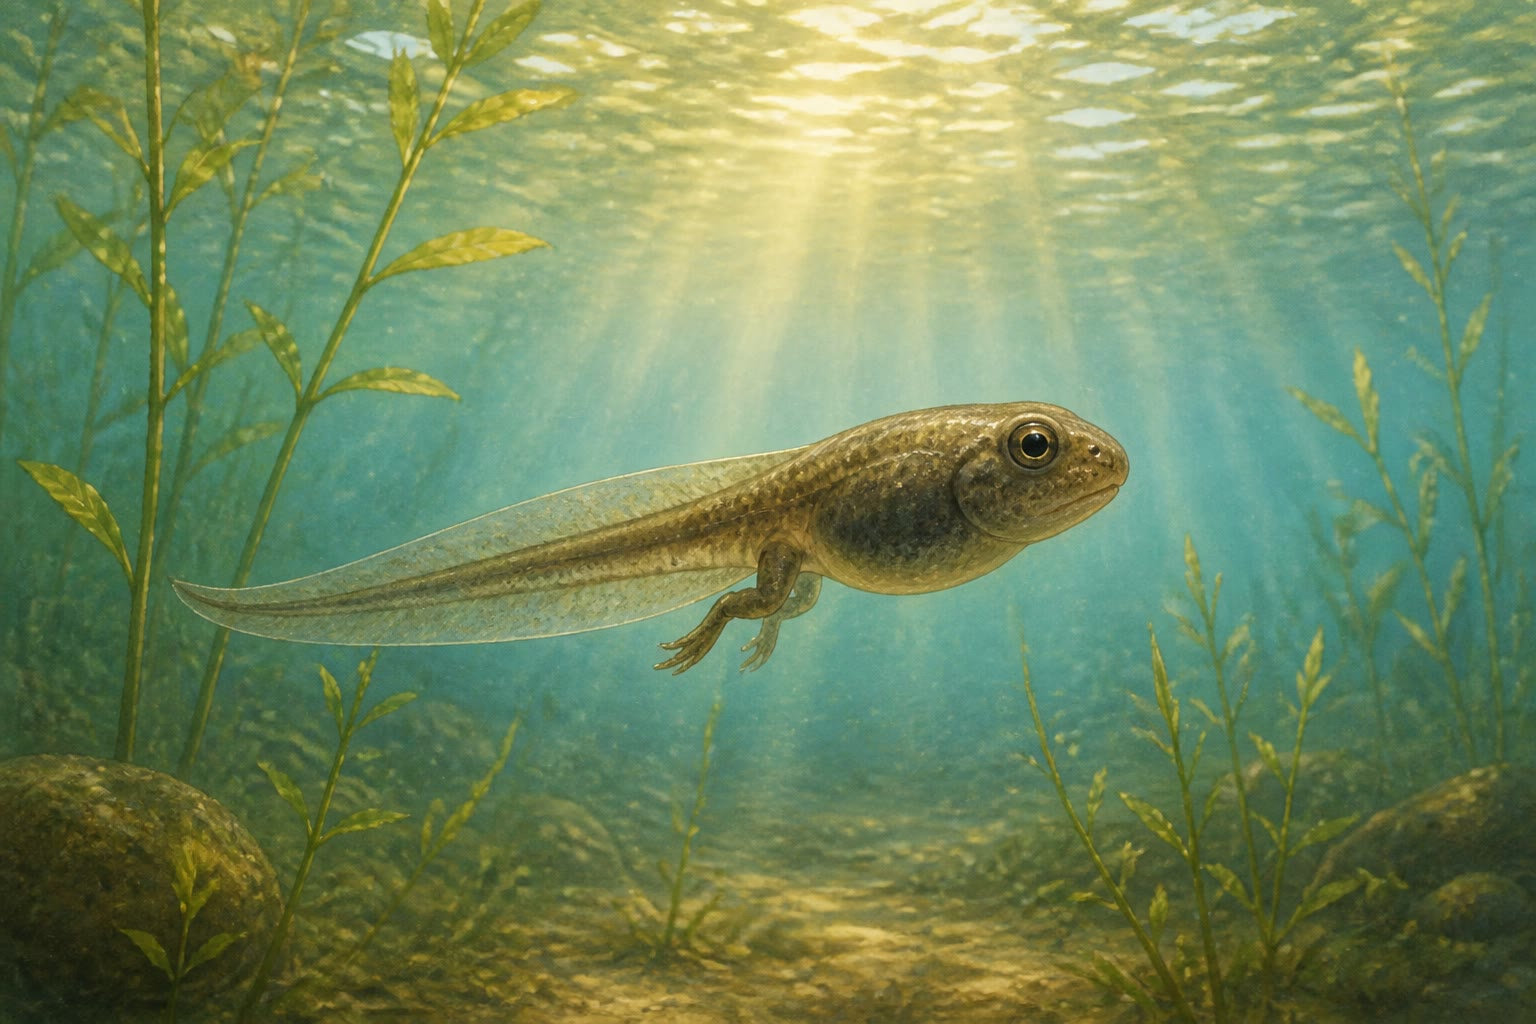
\includegraphics[width=0.6\linewidth]{images/book1/ai/g2-grow-tadpole.jpg}

{\small Surpris en pleine \omterm{def:g2:animals-grow-up:metamorphosis}{métamorphose}~: les pattes arrière ont
poussé, les pattes avant sont encore à venir, la queue est encore
longue.}
\end{omfigure}

\begin{omfigure}
\begin{tikzpicture}
  \node[anchor=south west, inner sep=0] (img) at (0,0)
    {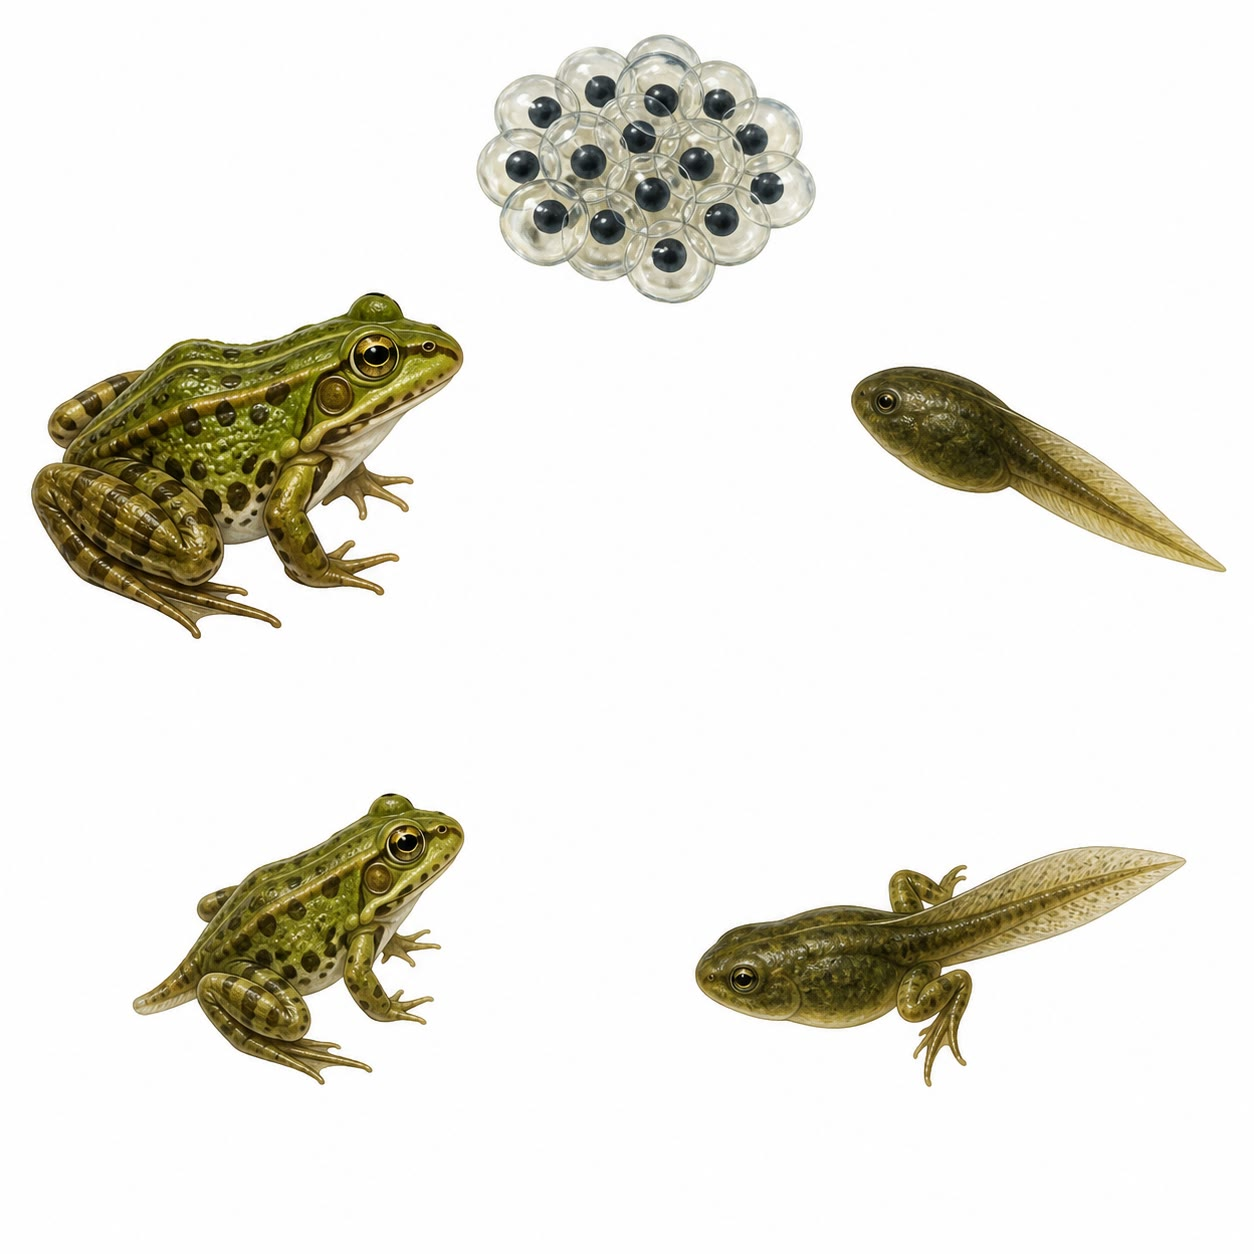
\includegraphics[width=0.72\linewidth]{images/book1/ai/fig-frog-cycle.jpg}};
  \begin{scope}[x={(img.south east)}, y={(img.north west)},
      every node/.style={font=\small}]
    \node[above] at (0.33,0.92) {les œufs dans la mare};
    \node[right, align=left] at (0.87,0.44)
      {têtard~:\\ une queue, pas de pattes};
    \node[below, align=center] at (0.80,0.05)
      {les pattes arrière poussent,\\ puis celles de devant};
    \node[below] at (0.22,0.05) {la queue disparaît~: un grenouillet};
    \node[left, align=right] at (0.075,0.78) {grenouille adulte};
    \draw[->, thick, omProp] (0.70,0.86) to[bend left=20] (0.87,0.68);
    \draw[->, thick, omProp] (0.88,0.38) to[bend left=15] (0.85,0.25);
    \draw[->, thick, omProp] (0.60,0.16) to[bend left=12] (0.42,0.14);
    \draw[->, thick, omProp] (0.16,0.32) to[bend left=15] (0.13,0.48);
    \draw[->, thick, omProp] (0.30,0.80) to[bend left=18] (0.42,0.88);
  \end{scope}
\end{tikzpicture}

{\small La \omterm{def:g2:animals-grow-up:metamorphosis}{métamorphose} de la grenouille, dans le sens des aiguilles
d'une montre à partir des \omterm{def:g2:animals-grow-up:born}{œufs}~: têtard, pattes, grenouillet, adulte
--- et l'adulte pond les \omterm{def:g2:animals-grow-up:born}{œufs} suivants.}
\end{omfigure}

\begin{example}[La route du papillon]\label{ex:g2:animals-grow-up:butterfly}
De l'\omterm{def:g2:animals-grow-up:born}{œuf} du papillon sort une \emph{chenille}\index{chenille}, qui
ne fait guère que manger des \omterm{def:g1:plants-around-us:parts}{feuilles} et grandir. Un jour, elle
s'enveloppe dans un étui, la \emph{chrysalide}\index{chrysalide}, et
cesse de bouger. À l'intérieur, le corps est reconstruit~; après
quelques semaines l'étui se fend, et il en sort un papillon qui
déplie ses ailes neuves et humides. \omterm{def:g2:animals-grow-up:born}{Œuf}, \omterm{ex:g2:animals-grow-up:butterfly}{chenille}, \omterm{ex:g2:animals-grow-up:butterfly}{chrysalide},
papillon~: quatre étapes d'un seul et même \omterm{def:g1:animals-around-us:animal}{animal}.
\end{example}

\begin{method}[Lire le cycle de vie d'un animal]\label{met:g2:animals-grow-up:read}
Pour n'importe quel \omterm{def:g1:animals-around-us:animal}{animal} que tu rencontres~:
\begin{enumerate}
  \item demande-toi comment il naît~: d'un \omterm{def:g2:animals-grow-up:born}{œuf}, ou vivant~?
  \item demande-toi à quoi ressemble le jeune~: à une miniature de
        ses parents, ou à une autre forme~?
  \item si la forme est autre, il se transformera~: cherche les
        étapes de sa \omterm{def:g2:animals-grow-up:metamorphosis}{métamorphose}~;
  \item dessine le cycle comme une roue, avec une flèche qui
        ramène de l'adulte aux \omterm{def:g2:animals-grow-up:born}{œufs}.
\end{enumerate}
\end{method}

\begin{remark}[Du lait, ou au travail tout de suite]\label{rem:g2:animals-grow-up:care}
Les chatons sont nourris et lavés par leur mère pendant des
semaines~; un têtard qui vient d'éclore ne reçoit aucune aide et
doit se nourrir seul dès le premier jour. Certains jeunes \omterm{def:g1:animals-around-us:animal}{animaux}
sont soignés, d'autres commencent leur vie seuls --- les deux routes
mènent à l'âge adulte.
\end{remark}

\section{Exercices}

\begin{exercise}[$\star$]\label{exo:g2:animals-grow-up:1}
Donne les deux façons dont les jeunes \omterm{def:g1:animals-around-us:animal}{animaux} viennent au monde,
avec un exemple de chacune.
\end{exercise}

\begin{exercise}[$\star$]\label{exo:g2:animals-grow-up:2}
D'un \omterm{def:g2:animals-grow-up:born}{œuf}, ou né vivant~: (a) un poussin~? (b) un chaton~? (c) une
grenouille~? (d) un lapin~? (e) un escargot~?
\end{exercise}

\begin{exercise}[$\star$]\label{exo:g2:animals-grow-up:3}
Que boit d'abord un chaton~? Quels \omterm{def:g1:animals-around-us:animal}{animaux} de ce chapitre boivent la
même chose à la \omterm{def:g2:born-grow-die:cycle}{naissance}~?
\end{exercise}

\begin{exercise}[$\star$]\label{exo:g2:animals-grow-up:4}
Qu'est-ce que la \omterm{def:g2:animals-grow-up:metamorphosis}{métamorphose}~? Nomme les deux exemples célèbres de
ce chapitre.
\end{exercise}

\begin{exercise}[$\star$]\label{exo:g2:animals-grow-up:5}
Range les étapes de la grenouille dans l'ordre~: grenouille ---
\omterm{def:g2:animals-grow-up:born}{œufs} --- têtard à pattes --- têtard.
\end{exercise}

\begin{exercise}[$\star$]\label{exo:g2:animals-grow-up:6}
Range les étapes du papillon dans l'ordre~: papillon --- \omterm{ex:g2:animals-grow-up:butterfly}{chenille}
--- \omterm{def:g2:animals-grow-up:born}{œuf} --- \omterm{ex:g2:animals-grow-up:butterfly}{chrysalide}. À quelle étape l'\omterm{def:g1:animals-around-us:animal}{animal} mange-t-il des
\omterm{def:g1:plants-around-us:parts}{feuilles} et grandit-il le plus~?
\end{exercise}

\begin{exercise}[$\star$]\label{exo:g2:animals-grow-up:7}
Quel jeune \omterm{def:g1:animals-around-us:animal}{animal} est une miniature de ses parents~: le têtard ou le
poulain~? Que veut dire grandir pour celui-là~?
\end{exercise}

\begin{exercise}[$\star$]\label{exo:g2:animals-grow-up:8}
Pourquoi la poule se pose-t-elle sur ses \omterm{def:g2:animals-grow-up:born}{œufs}~? Que s'y passe-t-il à
l'intérieur, d'après \cref{rem:g2:animals-grow-up:egg}~?
\end{exercise}

\begin{exercise}[$\star\star$]\label{exo:g2:animals-grow-up:9}
Dans la mare, Zoé trouve un petit \omterm{def:g1:animals-around-us:animal}{animal} à tête ronde, longue queue,
deux pattes arrière et sans pattes avant. À l'aide de la figure du
cycle de la grenouille, dis exactement où il en est sur sa route, ce
qu'il était avant, et ce qui vient ensuite.
\end{exercise}

\begin{exercise}[$\star\star$]\label{exo:g2:animals-grow-up:10}
«~La \omterm{ex:g2:animals-grow-up:butterfly}{chenille} est morte dans son étui, et un papillon est venu s'y
installer.~» Que s'est-il vraiment passé dans la \omterm{ex:g2:animals-grow-up:butterfly}{chrysalide}~?
Réponds avec \cref{def:g2:animals-grow-up:metamorphosis} et
\cref{ex:g2:animals-grow-up:butterfly}.
\end{exercise}
